
\section{Introduction}
In the enchanting world of wizardry, the concoction of potions and elixirs stands as a fundamental practice \cite{personalgrimoires2013}. This chapter delves into the ancient recipes, mystical ingredients, and brewing techniques that define the art of potion-making. From healing draughts to transformative elixirs, we embark on a magical journey through the alchemical mysteries that lie within the cauldron.

In the realm of potion-making, precise measurements and careful concoction are essential. Wizards often use enchanted cauldrons and stirring wands to brew elixirs with specific effects. For example, a healing potion might require precisely \SI{100}{\milli\liter} of phoenix tears, while a transformative elixir might demand \SI{50}{\gram} of dragon scale powder.

\section{Foundations of Potion-Making}

The foundation of potion-making lies in the understanding of magical ingredients (Tbl.~\ref{tbl:potions}), their properties, and the precise art of brewing \cite{rareingredients2020}. This section explores the essential components that contribute to the success of potions, emphasizing the delicate balance required to create elixirs with specific effects. From rare herbs to the tears of mythical creatures, each ingredient plays a crucial role in the alchemical dance of potion-making.

Understanding the magical properties of ingredients is crucial. Rare herbs like moonstone essence or wyvern claw essence contribute unique effects to potions. For optimal results, the brewing process involves heating the mixture to \SI{200}{\celsius} under the light of a waxing moon.

\begin{table}
\begin{center}
\begin{tabular}{ l l l }
\hline
\textbf{Rare Ingredient} & \textbf{Magical Property} & \textbf{Elixir Examples} \\
\hline
Moonstone Essence & Lunar Enhancement & Lunar Tonic \\
Dragon Scale Powder & Elemental Resilience & Draconic Invigoration \\
Mermaid Tears & Water Manipulation & Oceanic Renewal \\
Phoenix Feather Extract & Healing Flames & Phoenix Rejuvenation \\
Wyvern Claw Essence & Potent Vigor & Wyrm's Vitality \\
\hline
\end{tabular}
\caption{\label{tbl:potions}The table highlights the efficacy of rare ingredients in potion brewing, showcasing their associated magical properties and providing examples of elixirs crafted with these ingredients. Potion-makers can refer to this table for guidance in selecting and combining rare components to achieve desired magical effects in their concoctions.}
\end{center}
\end{table}

\section{Classification of Potions}

\begin{figure}
    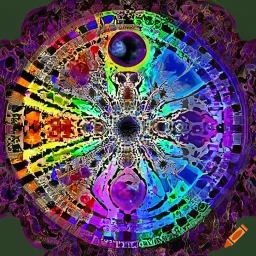
\includegraphics[width=\textwidth]{fig/img2.png}
    \caption{Moonfire's Elixir Spectrum \cite{moonfireelixirs2023} is a color-coded chart showcasing the diverse range of potions and elixirs crafted by Potion Mistress Isabella Moonfire. Each hue represents a unique category of magical concoctions, while the intertwining lines highlight the synergies between key ingredients. This visual guide aids potion-makers in understanding the alchemical balance required for successful brews.}
    \label{fig:img2}
  \end{figure}

Potions and elixirs come in diverse forms (Fig.~\ref{fig:img2}), each designed for specific magical purposes. This section categorizes potions based on their intended effects, creating a comprehensive classification system. From healing potions that mend wounds to polyjuice potions that enable transformation, wizards gain insights into the wide array of magical concoctions and their applications.

Potions can be categorized based on their effects. Healing potions are often denoted with a blue hue, while transformative elixirs emit a radiant glow. This classification system aids wizards in selecting the right potion for various magical needs.


\section{Brewing Techniques and Apparatus}
The art of potion-making extends beyond ingredient selection to the precise brewing techniques and magical apparatus used in the process \cite{potionbrewingtechniques2017}. This section explores the enchanted cauldrons, stirring \glspl{wand}, and heating charms that aid wizards in creating potent elixirs. Wizards often use the \gls{pot} to brew mystical elixirs. The chapter also delves into the significance of lunar cycles and celestial alignments in optimizing potion brewing for maximum efficacy.

The choice of cauldron and \gls{wand}, along with the correct application of heating charms, plays a significant role. Enchanted apparatus ensures the brewing process is precise and efficient. Wizards meticulously follow procedures to achieve the desired magical potency in their elixirs.

\section{Experimental Alchemy}
Wizards often push the boundaries of traditional potion-making through experimental alchemy \cite{darkartselixirs2015}. This section investigates the methods employed to discover new potion recipes, modify existing ones, and explore the uncharted territories of magical mixology. From the creation of innovative elixirs to the study of magical side effects, experimental alchemy opens new doors for wizards seeking to expand their knowledge of potion-making.

In the pursuit of innovation, wizards engage in experimental alchemy. This involves testing new ingredients and altering brewing techniques. Wizards might experiment with varying quantities of rare substances to discover unique elixirs or study the effects of lunar cycles on potion efficacy.

\section{Conclusion}
As we conclude our exploration into potions and elixirs, we reflect on the magical alchemy that has been unveiled in this chapter. The intricate dance of ingredients, the classification of effects, and the experimental pursuits contribute to the rich tapestry of potion-making. The insights gained serve as a foundation for further magical research, encouraging wizards to continue their journey into the captivating world of alchemical wonders.


